\documentclass[17pt,a4paper,notitlepage]{article}
\pagestyle{plain}
%\usepackage[retainorgcmds]{IEEEtrantools}
\usepackage{amsmath}
\usepackage{amsthm}
\usepackage{graphicx}
%\usepackage{extsizes}
%\usepackage[font=small]{caption}\textsc{\textsc{}}
\usepackage{url}
\usepackage{natbib}
\bibliographystyle{plainnat}
\usepackage{hyperref}
\usepackage[absolute]{textpos}
\setlength{\TPHorizModule}{1mm}
\setlength{\TPVertModule}{1mm}
%\usepackage[toc,page]{appendix}
%\usepackage{algorithm}
%\usepackage[noend]{algpseudocode}
%\usepackage{tikz}
%\usetikzlibrary{arrows}
\usepackage{algorithm2e}

\usepackage[left=2cm,top=2cm,right=2cm]{geometry}

\begin{document}

\title{Statistical methods to estimate the mean annual Emission Factor of a  fuel gas stream with variable composition. }
\author{DRAFT  Stijn Bierman, GSNL-PTX D/S}
\date{\today}
\maketitle

\abstract{Precise estimates of greenhouse gas emissions of refineries are required for regulatory compliance and to measure improvements in terms of reduced net emissions. For example, refineries in The Netherlands which want to take part in $\text{CO}_2$ emissions trading are required by the Dutch Emissions Authority (NEA) to report estimates of the annual average Emission Factor (EF; the amount of produced $\text{CO}_2$ per amount of combusted fuel gas) of each refinery fuel gas. 
	
The composition of refinery fuel gases, and therefore also the EF, varies with time. The EF of a sample, taken from the flow of a refinery fuel gas, can be measured in the laboratory. The cost per sample is relatively high, and a large number of samples is typically required to estimate the annual average EF with sufficient precision. For the same number of laboratory samples, more precise estimates can be obtained if an auxiliary variable is available which correlates strongly enough with laboratory measurements of EF and can be measured at low cost and high frequency. Ideally, an auxiliary variable can be measured continuously using an online measurement device which is permanently in place. 

An overview is given of statistical recipes (estimators) which yield estimates of the annual average EF and associated precision, based on laboratory measurements alone or on a combination of laboratory measurements and one or more continuously monitored auxiliary variables. Estimators are compared in terms of their uncertainty, measured by the width of the 95\% confidence interval of the mean, and their coverage probability, i.e. the proportion of cases in which the confidence interval contains the true average EF. This is done using a simulation study. 

The uncertainty of the estimate of the annual average EF depends on sample size as well as on the process variability in EF The use of an auxiliary variable greatly increases the precision of estimates. Bootstrap estimators have good performance, and can readily be extended to multiple regression in case multiple auxiliary variables are required to get predicted EF which correlates strongly with EF. 

In a study of a fuel gas in Pernis, EF was found to correlate strongly with Stoichiometric Air Requirement (SAR) and Lower Heating Value (LHV). Models which combine either SAR or LHV with molar mass can predict EF to a high precision. Molar mass is currently already measured online. If additional online measurements can be done which correlate with either SAR or LHV (or which measure these variables directly), such as a calorimeter or oxygen content, then this could greatly improve the estimates of annual average EF for fuel gas in Pernis.
}

\clearpage
\tableofcontents  % Mandatory item, do not remove it.
\listoffigures    % This can be remarked out if not needed.
\listoftables     % This can be remarked out if not needed.

\clearpage
\section{Introduction}\label{Intro}

Trustworthy and precise estimates of greenhouse gas emissions of refineries and petrochemical plants are essential to measure reductions in net emissions per amount of produced product and to demonstrate regulatory compliance. For example, refineries in The Netherlands which want to take part in $\text{CO}_2$ emissions trading, are required by the Dutch Emissions Authority (NEA) to report estimates of the annual average Emission Factor (EF; the amount of produced $\text{CO}_2$ per amount of combusted fuel gas; see e.g. \cite{API2009}) of each fuel gas. For each fuel gas stream, the annual average EF can be multiplied with the annual total amount of combusted fuel gas to yield an estimate of the total amount of $\text{CO}_2$ produced. The NEA requires these estimates of annual average EF to have an associated minimum precision. 

The EF of a single sample, taken from the flow of a fuel gas, can be measured in the laboratory. The cost per sample is relatively high, and a large number of samples may be needed to estimate the annual average EF with sufficient precision. A well known and potentially highly efficient way to more precise estimates, for the same number of laboratory samples, is to use one or more auxiliary variables which correlate with laboratory measurements of EF and which can be measured at lower cost and higher frequency (see e.g. chapters 6 and 7 in \cite{Cochran77} and chapters 7 and 8 in \cite{Thompson}). Ideally, an auxiliary variable correlates strongly with EF and can be measured continuously using an online measurement device which is permanently in place. The auxiliary variables are not of direct interest themselves, but can help in obtaining estimates with higher precision.

A large body of scientific literature exists on how to estimate means or totals based on samples and auxiliary variables. Excellent overviews are given by \citet{Cochran77} and \citet{Thompson}. Few people are familiar with this literature, and there are no universally applicable rules which produce valid and efficient estimates in all situations. It is not straightforward to select an appropriate statistical procedure for a given situation, and to transparently demonstrate that the assumptions are met for the method to yield valid estimates. It seems worthwhile therefore to build up a body of knowledge on appropriate statistical methodology which may be used to obtain such estimates. 

This report provides and overview of statistical recipes (estimators) which yield estimates of the annual average EF and associated precision, based on laboratory measurements alone or on a combination of a continuously monitored auxiliary variable and laboratory measurements. The estimators are applied to synthetic data sets, generated under scenarios which capture a range of different situations which may be encountered in practice. The scenarios are defined in terms of: 
\begin{itemize}
	\item The number of laboratory measurements
	\item The correlation (strength of relationship) between the auxiliary variable and the laboratory measurements
	\item The variability in EF, auxiliary variable and flow rate measurements (due to a combination of process variability and measurement errors)
	\item The correlation (strength of relationship) between flow rate and EF, and between flow rate and auxiliary variable
\end{itemize} 

Estimators are compared in terms of their precision, measured by the width of the 95\% confidence interval of the mean, and their coverage probability, i.e. the proportion of cases in which the confidence interval contains the true average EF. If an estimator produces confidence intervals with a coverage probability (substantially) below 95\%, then the  precision estimates based on this estimator are unjustifiably high and as such potentially misleading. For each scenario, the most efficient estimator yields an estimate with the highest precision whilst maintaining an acceptable coverage probability. 

\clearpage
\section{Estimators}\label{Estimators}
 
Let $y_i$ be the EF as measured in the laboratory on sample $i$; $i=1,2,\ldots ,n$, where $n$ denotes the number of samples taken from the fuel gas flow during the year (the sample size). Triples of laboratory (EF; $y_i$), auxiliary ($x_i$) and flow rate ($b_i$) measurements at the time that sample $i$ was taken are denoted by: $(y_i,x_i,b_i)$. The assumption is that measurements of the flow rate and auxiliary variable are always available at the time a sample was taken. Let $X_{j}$ and $B_j$ be a measurement of an auxiliary variable and flow rate respectively, where $j=1,2,\ldots,k$ is the total number of measurements of this auxiliary variable taken on the fuel gas flow during the year. Typically, $k \gg n$, because the auxiliary variable and flow rate can be measured at high frequency at relatively low cost. 

Below, a number of statistical procedures (estimators) are given for estimating the annual average EF, $\bar{y}$, and the lower and upper bound of the 95\% confidence interval, $\bar{Y}_{L}$ and $\bar{Y}_{U}$ respectively. The width $U$ of the confidence interval is given by $U=\bar{Y}_{L}-\bar{Y}_{U}$. The relative precision,$\%U$, of the estimate $\bar{y}$ is given by half the width of the confidence interval divided by the estimate of the annual average: $\%U=100\frac{U}{2\bar{y}}$.

\subsection{Without auxiliary variable: Simple Random Sampling (SRS)}\label{SRS}
If no auxiliary variable is available, and assuming that a representative sample of the fuel gas flow has been taken, the annual average EF can be estimated as:
\begin{equation}\label{eqn:SRS}
\bar{y}=\Sigma_{i=1}^{n}(y_i w_i),
\end{equation}
where $w_i$ is given by:
\begin{equation}\label{eqn:weights}
w_i=\frac{b_i}{\Sigma_{i=1}^{n}b_i}.
\end{equation}

Samples can be taken at regular time intervals, as long as it can be demonstrated that there are no periodic trends in the EF that coincide with the sampling frequency. A simple time series plot of EF measurements is informative: if there are no apparent time-trends then more or less regular sampling during the year is acceptable. If there are large gaps during the year, e.g. of one or more months without any samples being taken and if there are (or may be) longer-term trends (lasting weeks and months) in EF, then the set of collected samples may no longer be representative for the annual average.

An estimate of the standard error of the weighted mean given by equation~\ref{eqn:SRS} is given by (see \cite{GATZ19951185} and \cite{Cochran77}):
\begin{equation}\label{eqn:varSRS}
s_{\bar{y}}=\sqrt{\frac{n}{n-1} \Sigma_{i=1}^{n}[w_i^2 (y_i-\bar{y})^2]}
\end{equation}

The upper and lower bound of the 95\% confidence interval are given by:
\begin{subequations}\label{eqn:ciSRS}
	\begin{align}
	\bar{y}_{L} &= \bar{y}-t_{0.975;n-1}s_{\bar{y}} \\
	\bar{y}_{U} &= \bar{y}+t_{0.975;n-1}s_{\bar{y}} ,
\end{align}
\end{subequations}
where $t_{0.975;n-1}$ is the 97.5 percentile of the t distribution with $n-1$ degrees of freedom.

\subsection{Without auxiliary variable: Bootstrap}\label{SRSBoot}
A non-parametric Bootstrap (see \cite{EfroTibs93}) method can be used to estimate the standard error or confidence interval of $\bar{y}$. Synthetic data sets are created by drawing samples at random with replacement from the observed set of samples. Each synthetic data set is of equal size to the observed data set, and consists of measurements that were present in the original (actual) data set, although not every measurement in the original data set may have been drawn for inclusion in the synthetic data set and other measurements may have been chosen more than once. The weighted mean is computed for each synthetic data set using equation~\ref{eqn:SRS}). This way, a statistical distribution of means is formed from which the 2.5 an 97.5 percentiles are taken as the lower and upper limits respectively of the 95\% confidence interval. Pseudocode with an outline of the Bootstrap procedure is given in Algorithm~\ref{PseudoBootSRS}.

\RestyleAlgo{boxruled}
\LinesNumbered
\DontPrintSemicolon
\SetKwFor{RepTimes}{repeat}{times}{end}
\begin{algorithm}[h] \label{PseudoBootSRS}
	\caption{Bootstrap estimate of the confidence interval of a weighted sample mean}
	\KwData{The set of $n$ pairs of measurements $(y_i,b_i)$}
	Initialization: Generate a sequence of integers $r={1,2,\ldots,n}$\;
	\RepTimes{M}{
		Generate a random set $r^*$ of indicators by drawing $n$ values at random with replacement from the set $r$\;
		Create a synthetic data set of $n$ pairs of values $(y_{r},b_{r})$, where the indicators $r$ are taken from the set $r^*$ which was created in the previous step\;
		Based on the synthetic data, compute the weighted sample mean  $\bar{y^*}=\frac{\Sigma(y_{r} b_{r})}{\Sigma b_{r}}$, and store this value in a vector\;
	}
	Rank the vector of size $M$ with sample means $\bar{y^*}$ from smallest to largest and take the 2.5 and 97.5 percentiles as estimates of the lower and upper bounds of the confidence interval of the mean respectively.
\end{algorithm}

Advantages of the Bootstrap:
\begin{itemize}
	\item The methodology is generic: any estimator for the mean may be used instead of the weighted mean.
	\item It is relatively straightforward to implement in a common data science language such as \textit{R}, \textit{Python} or \textit{Matlab}.
	\item If the sample size is large enough (a rule of thumb is more than $n=50$ measurements for a reasonably symmetric distribution of values), and the measurements are independent and representative draws from the population, then this method will tend to yield reasonable estimates with good coverage probability.
\end{itemize}

The main disadvantages of the Bootstrap are:
\begin{itemize}
	\item It is a computationally intensive method.
	\item This method does not work well with small sample sizes (e.g. less than $n=50$ samples).
	\item The assumptions under which the results are valid are less explicit compared to a fully parametric method.
\end{itemize}

\subsection{With a single auxiliary variable: regression estimator as in Cochran, 1977}\label{AuxCochran}

The linear regression estimator is designed to increase precision by use of an auxiliary variable $x$ which is correlated with the actual variable of interest $y$ (\cite{Cochran77}, page 189). For this estimator, it is assumed that the annual average of the auxiliary variable $\bar{X}$ is known:
\begin{equation}\label{eqn:barbigX}
\bar{X}=\frac{\Sigma_{j=1}^k B_j X_j}{\Sigma_{j=1}^k B_j} 
\end{equation}
This is reasonable only when both the auxiliary variable and flow rate are monitored continuously and at high frequency during the entire year, and a value is stored for example every hour or every 15 minutes.

The linear regression estimate of the annual average EF is given by:
\begin{equation}\label{eqn:lr}
\bar{y}_{lr}=\bar{y}+a_1(\bar{X}-\bar{x}),
\end{equation}
where the subscript $lr$ denotes \textit{linear regression} and $a_1$ is the slope of a linear regression line as an estimate of the increase in $y$ for a unit increase in the value of $x$ (see equation 7.1 in \cite{Cochran77}). In equation~\ref{eqn:lr}, $\bar{x}$ is the weighted sample mean of the auxiliary variable:
\begin{equation}\label{eqn:barx}
\bar{x}=\Sigma_{i=1}^{n}(x_i w_i),
\end{equation}
with the $w_i$ as given in equation~\ref{eqn:weights}.

The parameter $a_1$ is obtained using the usual least squares estimator:
\begin{equation}\label{eqn:b}
a_1=\frac{\Sigma_{i=1}^n[(y_i-\hat{y})(x_i-\hat{x})]}{\Sigma_{i=1}^n[x_i-\hat{x}]^2},
\end{equation}
where $\hat{y}=n^{-1}\Sigma y_i$ and $\hat{x}=n^{-1}\Sigma x_i$ are simple unweighted arithmetic means.

The rationale behind the estimator as given in equation~\ref{eqn:lr} is that if due to random sampling variability $\bar{x}$ is below the annual average $\bar{X}$, then the expectation is that estimate $\bar{y}$ will be below average by an amount $a_1(\bar{X}-\bar{x})$ (\cite{Cochran77}, page 189).
We note that the estimator given in equation~\ref{eqn:lr} is not identical to equation 7.1 in \cite{Cochran77} because of the use of a weighted arithmetic mean instead of a simple arithmetic mean.

An estimate of the standard error of $\bar{y}_{lr}$ is given by equation 7.29 in \citet{Cochran77}:
\begin{equation}\label{eqn:varlr}
s_{\bar{y}_{lr}}=\sqrt{ \frac{1}{n-2} \Sigma_{i=1}^{n}[(y_i-\bar{y}_{lr})(x_i-\bar{x})]^2 }
\end{equation}

The upper and lower bound of the 95\% confidence interval are given by:
\begin{subequations}\label{eqn:cilr}
	\begin{align}
	\bar{y}_{L} &= \bar{y}_{lr}-t_{0.975;n-2}s_{\bar{y}_{lr}} \\
	\bar{y}_{U} &= \bar{y}_{lr}+t_{0.975;n-2}s_{\bar{y}_{lr}} ,
	\end{align}
\end{subequations}
where $t_{0.975;n-2}$ is the 97.5 percentile of the t distribution with $n-2$ degrees of freedom.

We note that the estimator of the standard error given by equation~\ref{eqn:varlr} does not take the variability in the flow rate measurements into account. %Another important thing to note is that all measurements must be from the year to which the estimate of the annual average EF applies.  %This estimator may therefore underestimate the width of the confidence interval, with consequent poor coverage probabilities, if the variability in flow rates is high.

\subsection{With a single auxiliary variable: regression estimator as in van Zanten, 2016}\label{AuxVZ}

A regression estimator for the average annual EF is described in \citet{vanZanten}:
\begin{equation}\label{eqn:vanzanten}
\bar{y}_{vz} = a_0 + a_1\bar{X},
\end{equation}
where the subscript $vz$ refers to the author of the technical report \citet{vanZanten}, $\bar{X}$ is given by equation~\ref{eqn:barbigX}. 

The parameters $a$ and $b$ are the intercept and slope respetively of a linear regression model, $y_i = a_0 + a_1 x_j + z_j$, where $z_j$ are stochastic variables that give the deviations between measured and predicted values. The $z_j$ are assumed to be independent and Normally (Gaussian) distributed. The slope parameter $a_1$ is given by equation~\ref{eqn:b}. The intercept $a_0$ is given by:
\begin{equation}\label{eqn:a}
a_0 = \hat{y}-a_1\hat{x},
\end{equation}
where $\hat{y}=n^{-1}\Sigma y_i$ and $\hat{x}=n^{-1}\Sigma x_i$ are simple unweighted arithmetic means.

The estimator for the standard error of $\bar{y}_{vz}$ is given in equation 7 in \citet{vanZanten}:
\begin{equation}\label{eqn:varvz}
s_{\bar{y}_{vz}}=s_{re} \sqrt{n^{-1} \frac{\Sigma_{i=1}^n [x_i-\bar{X}]^2}{\Sigma_{i=1}^n [x_i - \hat{x}]^2} + m^{-1} \left( 1 + \frac{k^{-1}\Sigma_{j=1}^k[B_j-\hat{B}]^2}{ (\hat{B})^2 } \right) },
\end{equation}
where $\hat{y}=n^{-1}\Sigma y_i$, $\hat{x}=n^{-1}\Sigma x_i$ and $\hat{B}=k^{-1}\Sigma B_j$ are simple unweighted arithmetic means. The standard deviation of the residuals of the linear regression model $s_{re}$ is given by:
\begin{equation}\label{eqn:sresiduals}
s_{re}=\sqrt{\frac{\Sigma_{i=1}^n[z_i-\hat{z}]^2}{n-2}},
\end{equation}
where $\hat{z}=n^{-1}\Sigma z_j$ is the simple unweighted arithmetic mean of the model residuals.

The upper and lower bound of the 95\% confidence interval are given by:
\begin{subequations}\label{eqn:civz}
	\begin{align}
	\bar{y}_{L} &= \bar{y}_{vz}-t_{0.975;n-2}s_{\bar{y}_{vz}} \\
	\bar{y}_{U} &= \bar{y}_{vz}+t_{0.975;n-2}s_{\bar{y}_{vz}} ,
	\end{align}
\end{subequations}
where $t_{0.975;n-2}$ is the 97.5 percentile of the t distribution with $n-2$ degrees of freedom.

It is not assumed that $\bar{X}$ is known without error. The variability in flow rate measurements is taken into account in the estimate of the standard error of the mean. %We note that it is assumed that the residuals of the regression model are not correlated with the flow rate.

\subsection{With a single or multiple auxiliary variables: regression estimator with Bootstrap}\label{AuxBoot}

The Bootstrap method, introduced in section~\ref{SRSBoot}, may also be applied to estimate the confidence interval of the mean based on a linear regression equation. Two variations of the algorithm are discussed:
\begin{itemize}
	\item A Bootstrap algorithm which assumes that the flow rate is not correlated with the EF and the auxiliary variable. In this algorithm, the EF is modelled as a linear function of the auxiliary variable only. 
	\item A Boostrap algorithm in which the EF is modelled as a linear function of the auxiliary variable and flow rate. This is applicable only in situations where the flow rate correlates with the EF and auxiliary variable. 
\end{itemize}
The second variation of the algorithm, with the linear regression of EF on both the flow rate and auxiliary variables, is included because the flow rate plays an important role in computing the weighted means and because the estimators in sections~\ref{AuxCochran} and~\ref{AuxVZ} do not take this possibility into account. A question of interest is therefore what the performance, in terms of coverage probabilities, of the estimators is when the flow rate correlates with the EF.
Pseudocode for the Bootstrap algorithm is given in Algrotihm~\ref{lrBoot1}.

The Bootstrap procedures outlined in this section can easily be extended to include more variables and slope parameters.

\RestyleAlgo{boxruled}
\LinesNumbered
\DontPrintSemicolon
\SetKwFor{RepTimes}{repeat}{times}{end}
\begin{algorithm}[h] \label{lrBoot1}
	\caption{Bootstrap estimate of the confidence interval of an estimate of the mean based on a linear regression equation of EF on the auxiliary variable (version 1) or both the auxiliary variable and flow rate (version 2).}
	\KwData{$n$ triples of measurements $(y_i,x_i,b_i)$; $k$ pairs of measurements ($X_j,B_j$); $k$ weights $W_j=\frac{B_j}{\Sigma_{j=1}^{k} B_j}$}
	Initialization: Generate a sequence of integers $r={1,2,\ldots,n}$\;
	\RepTimes{M}{
		Generate a random set $r^*$ of indicators by drawing $n$ values at random with replacement from the set $r$\;
		Create a synthetic data set of $n$ pairs of values $(y_{r},x_{r})$, where the indicators $r$ are taken from the set $r^*$ which was create in the previous step\;
		\If{regression model based on auxiliary variable}{
			Based on the synthetic data compute the intercept $a_0^*$ and slopes $a_1^*$ of the  linear regression equation $y_r=a_0^*+a_1^* x_r+z_r$ (using the standard least squares estimator for these parameters)\;
			Compute the standard deviation of the residuals of the regression model, $s^*_{re}$ \;
			Create a synthetic data set of $j=1,2,\ldots,k$ estimates of EF, $q_j$: $q_j=a_0^* + a_1^* X_j + z^*_j$, where the $z^*_j$ are drawn at random from a Normal distribution with mean zero and standard deviation $s^*_{re}$\;
		}
		\If{regression model based on auxiliary variable and flow rate}{
			Based on the synthetic data compute the intercept $a_0^*$ and slopes $a_1^*$ and $a_2$ of the  linear regression equation $y_r=a_0^*+a_1^* x_r+a_2^* b_r+z_r$ (using the standard least squares estimator for these parameters)\;
			Compute the standard deviation of the residuals of the regression model, $s^*_{re}$ \;
			Create a synthetic data set of $j=1,2,\ldots,k$ estimates of EF, $q_j$: $q_j=a_0^* + a_1^* X_j +a_2^* B_j + z^*_j$, where the $z^*_j$ are drawn at random from a Normal distribution with mean zero and standard deviation $s^*_{re}$\;
			
		}
		Based on the synthetic set of measurements $q_j$ compute the weighted mean $\bar{y^*}=\Sigma_{j=1}^{k}[W_jq_j]$ and store this value in a vector.
	}
	Rank the vector of size $M$ with sample means $\bar{y^*}$ from smallest to largest and take the 2.5 and 97.5 percentiles as estimates of the lower and upper bounds of the confidence interval of the mean respectively.
\end{algorithm}

\citet{Thompson} (chapter 8) outlines a number of estimators based on multiple regression, and mentions that more research is needed on the topic (page 117 in \cite{Thompson}). For this reason, it may best to use the Bootstrap to estimate uncertainties for multiple regression models.



\clearpage
\section{Model Validation}\label{Validation}

\subsection{Representativeness of the sample}

Samples can be taken at regular time intervals, as long as it can be demonstrated that there are no periodic trends in the EF that coincide with the sampling frequency. A simple time series plot of EF measurements is informative: if there are no apparent time-trends then more or less regular sampling during the year is acceptable. If there are large gaps during the year, e.g. of one or more months without any samples being taken and if there are (or may be) longer-term trends (lasting weeks and months) in EF, then the set of collected samples may no longer be representative for the annual average.

\subsection{Validity of the regression model}
More precise estimates can be obtained with auxiliary variables. However, the validity of these estimates depends to a large extent on the validity of the regression model (see for example chapter 4 in \cite{vanZanten}). Deviations of measurements from the regression line are assumed ot be independent and Normally distributed variables, with constant variance across the range of predicted values. A number of diagnostic plots can be used to assess whether these assumptions are reasonable, or to see if there are indications that they are violated.
\begin{itemize}
	\item Time series plots of model residuals should show no apparent patterns. If there are pattterns, then it is worth investigating whether or nor the residuals correlate with other variables (if available).
	\item A Quantile-Quantile plot to check if the model residuals are (at least approximately) normally distributed
	\item A scatterplot of predicted versus observed values, to check for potential outliers, and to see of the variability (the ``scatter'' around the 1:1 line) is roughly constant across the predicted range of values.
\end{itemize}

A good graphical analysis of the residuals is key for a good appraisal of the validity of the model.
\clearpage
\section{Assessment of the performance of estimators using a simulation study}\label{Simulation}

\subsection{Simulation method}
A simulation study, in which synthetic data with characteristics that are as close as possible to those that may occur in real life, may be used to better understand of  performance of the estimators presented in chapter~\ref{Estimators} in terms of:
\begin{itemize}
	\item The dependence of the precision (the width of the 95\% confidence interval) of the estimates, as a function of sample size, variability in the key process parameters (EF and flow rate) and the strength of the relationship between auxiliary variable and EF
	\item The coverage probability of the 95\% confidence intervals, measured by the proportion of times that the confidence intervals contain the true value of the annual average EF used to generate the synthetic data sets. 
\end{itemize}

An estimator yields valid results only if its associated coverage probability is (close to) 95\%. A good, or efficient, estimator yields, for a given sample size and scenario, a small width of the confidence interval whilst maintaining good coverage probability. If a high precision (small width of confidence interval) is associated with a coverage probability that is too low, then the precision estimate is misleading.

Scenarios are defined by a combination of the following:
\begin{itemize}
	\item The number of laboratory measurements
	\item The correlation (strength of relationship) between the auxiliary variable and the laboratory measurements
	\item The variability in EF, auxiliary variable and flow rate measurements (due to a combination of process variability and measurement errors)
	\item The correlation (strength of relationship) between flow rate and EF, and between flow rate and auxiliary variable
\end{itemize} 

It is assumed that the flow rate and auxiliary variable is monitored continuously, so that the uncertainty regarding for example the average, or weighted average, of the flow rate and auxiliary variable is negligible. At the point of writing this report, only a single auxiliary variable is used in the simulation study. 

Many synthetic data sets are created, each with $4\times24\times365=35040$ triples of measurements $(Y_j,B_j,X_j)$, representing a hypothetical situation in which all variables of interest were monitored every 15 minutes during the entire year. 
The true value of the annual average EF is taken to be:
\begin{equation*}
\mu_{true} = \frac{\Sigma[Y_jB_j]}{\Sigma B_j}.
\end{equation*}
The triples of measurements are drawn from a Multivariate Normal (MVN) distribution:

\begin{equation}\label{DrawMVN}
\begin{bmatrix}
Y \\
X \\
B
\end{bmatrix} \sim
\text{MVN} \left( 
\begin{bmatrix}
\mu_Y \\
\mu_X \\
\mu_B
\end{bmatrix},
\begin{bmatrix}
\sigma_{Y}^2 & \rho_{YX}\sigma_{Y}\sigma_{X} & \rho_{YB}\sigma_{Y}\sigma_{B} \\
\rho_{YX}\sigma_{Y}\sigma_{X} & \sigma_{X}^2 & \rho_{XB}\sigma_{X}\sigma_{B} \\
\rho_{YB}\sigma_{Y}\sigma_{B} & \rho_{XB}\sigma_{X}\sigma_{B} & \sigma_{B}^2 \\
\end{bmatrix}
\right),
\end{equation}
where ($\mu_y$,$\sigma_{Y}^2$), ($\mu_x$,$\sigma_{X}^2$) and ($\mu_B$,$\sigma_{B}^2$) are parameters for the mean and variance of the EF, auxiliary variable and flow rate respectively, to be specified to define a scenario. The parameters $\rho_{YX}$, $\rho_{YB}$ and $\rho_{XB}$ denote the correlation between the pairs of variables. In the simulation study,  $\rho_{YX}$ and $\rho_{YB}$ can be set independently, but $\rho_{XB}$ is set to be $\rho_{XB}=\rho_{YX}*\rho_{YB}$. The mean and variance of the auxiliary variable are of no consequence to the estimates as long as this variable is monitored continuously.

The sampling of the fuel gas flow is simulated by drawing $n$ triples $(y_j,b_j,x_j)$ at random without replacement from the set of $k$ triples $(Y_j,B_j,X_j)$.

An outline of the simulation procedure is given in pseudocode in Algorithm~\ref{sims}.

\RestyleAlgo{boxruled}
\LinesNumbered
\DontPrintSemicolon
\SetKwFor{RepTimes}{repeat}{times}{end}
\begin{algorithm}[h] \label{sims}
	\caption{Simulation study to estimate the relative precision and coverage probability of the estimators.}
	Initialize: Choose values for the sample size $n$, the pairs of values for the mean ad variance of the process parameters  ($\mu_y$,$\sigma_{Y}^2$), ($\mu_x$,$\sigma_{X}^2$) and ($\mu_B$,$\sigma_{B}^2$), and the correlation parameters $\rho_{YX}$ and $\rho_{YB}$. Set $I \gets 0$\;
	\RepTimes{M}{
		Generate a synthetic data set of 35040 triples $(Y_j,B_j,X_j)$ using equation~\ref{DrawMVN}.\;
		Compute the true value $\mu_{true}$.\;
		Generate a synthetic sample data set of $n$ triples $(y_j,b_j,x_j)$ by sampling at random without replacement.\;
		Apply the estimators described in chapter~\ref{Estimators} and store the estimated relative precision in a vector.\;
		\If{$\mu_{true}$ is smaller than the upper bound and larger than the lower bound of the 95\% confidence interval}{$I \gets I + 1$}
	}
	Rank the vector of size $M$ with precisions from smallest to largest and take the 2.5 and 97.5 percentiles as estimates of the range of values that the relative precision could take under the defined scenario. The coverage probability $C$ (expressed as a percentage) is given by $C=100 I/M$.
\end{algorithm}

The reliability of the coverage probability $C$ depends on the number of simulations $M$. To assess the uncertainty in the coverage probability due to small number of simulations, a 95\% confidence interval is computed based on the 2.5 and 97.5 percentiles of the Beta distribution: $\text{Beta}(I,M-I)$. 

\subsection{web-App to explore the expected precision of estimates for different sccenarios}\label{webApp}

A simple web-App has been created which allows the user to specify the scenario in terms of the key parameters of interest (see a screen shot of the web-App in figure~\ref{fig:App}):
\begin{itemize}
	\item The sample size $n$.
	\item The mean and standard deviation (defining process variability) of the EF, $\mu_{Y}$ and $\sigma_Y$.
	\item The mean and standard deviation (defining process variability) of the flow rate, $\mu_{B}$ and $\sigma_B$.
	\item The correlation between the auxiliary variable and the EF, $\rho_{XY}$.
	\item The correlation between the flow rate and the EF, $\rho_{YB}$.
\end{itemize}

the use must choose values for these parameters so that synthetic data sets are created that closely resemble the real-life situations.

Additionally, the following must be specified:
\begin{itemize}
	\item The number of simulations (synthetic data sets). The larger the number of simulations, the more precise the estimates of the performance of the estimators will be. For the relative precision, 500 simulations is typically sufficient. For a good estimate of coverage probability, typiclly at least 1000 simulations are required.
	\item A tick box to indicate whether or not Bootstrap estimators should be included. This is computer intensive, and it may take several minutes for the results to be generated.
	\item The number of simulations in the Bootstrap. For a reasonable assessment of the performance of the Bootstrap, at least 1000 simulations are required. The larger the number of Bootstrap simulations and synthetic data sets, the longer it will take for the results to be generated.
\end{itemize}

\begin{figure}[h]
	\centering
	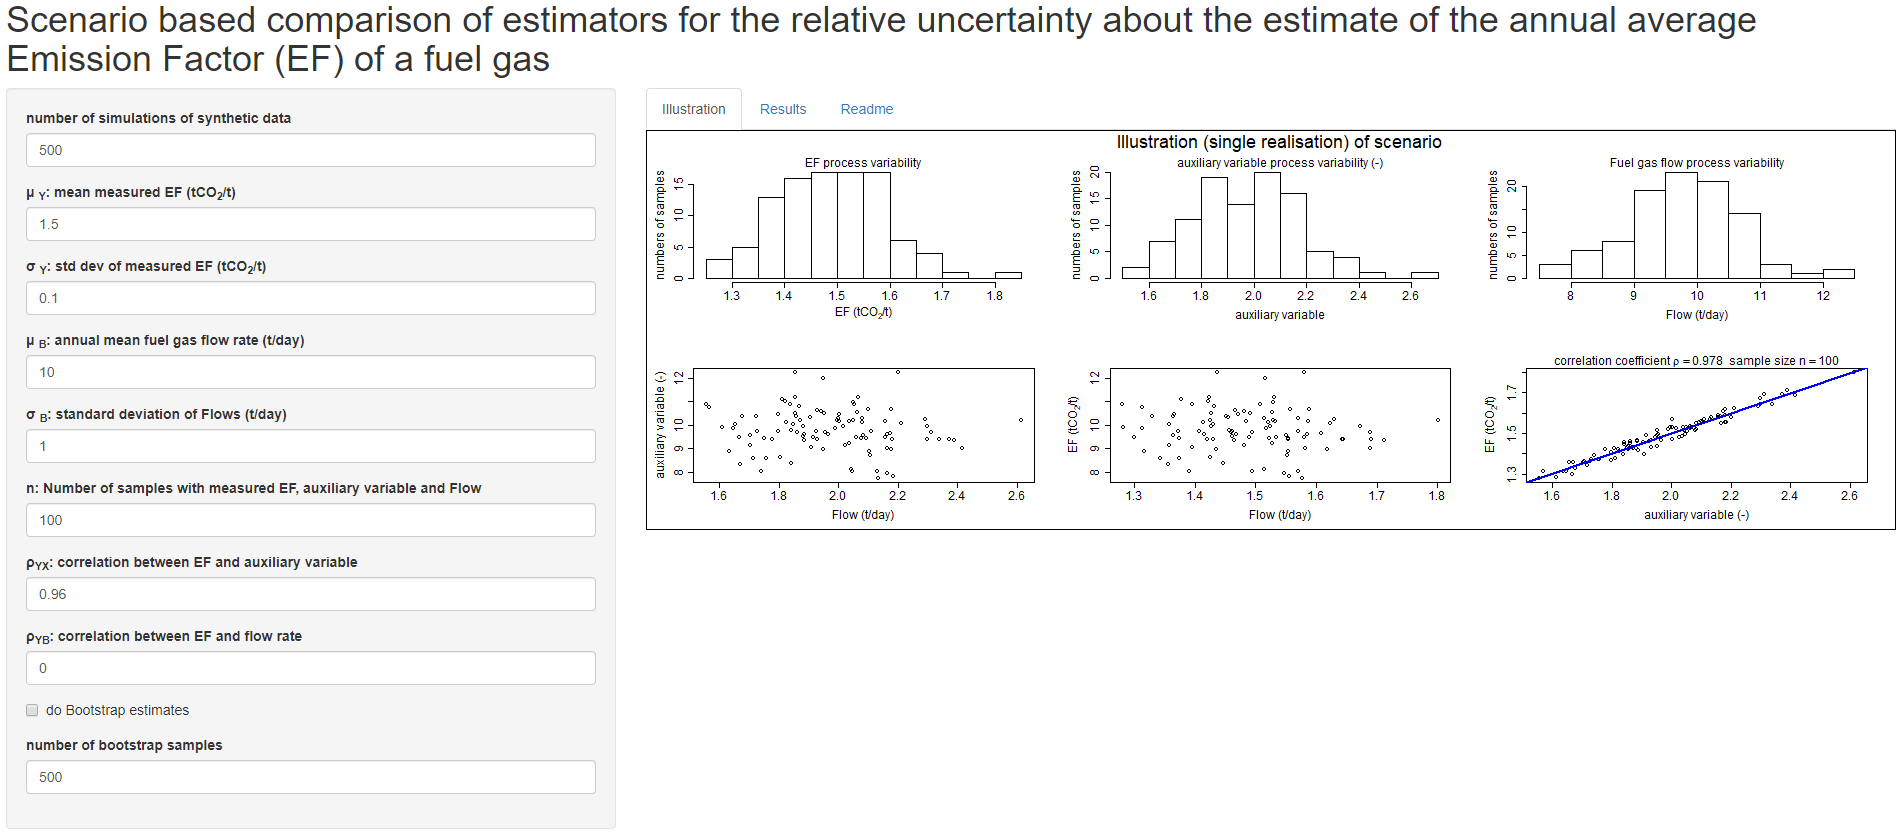
\includegraphics[width=\textwidth]{graphs/AppCapture.PNG}
	\caption{Screen shot of the web-App. On the left are the inputs that define the scenario as well as the number of required simulations. On the right are a number of graphs that illustrate, for a single synthetic data set, what the synthetic data look like. }
	\label{fig:App}
\end{figure}

An illustration of the results of the web-App, for a given scenario with $n=100$ and $\rho_{YX}=0.94$ is given in figure~\ref{fig:AppResults}. For this particular scenario, the estimators without auxiliary variable yield relative uncertainty estimates that are between 2.18\% and 3\%, well above the target set by the NEA of 0.5\%. The corresponding coverage probability is on target: close to 95\%. There is good agreement between the  Bootstrap (section~\ref{SRSBoot}) and Simple Random Sample (SRS; section~\ref{SRS}) estimators. The estimators with auxiliary variables (sections~\ref{AuxBoot},\ref{AuxCochran} and \ref{AuxVZ} all agree well in terms of both relative uncertainty and coverage, and yield uncertainty estimates in the range 0.62\% - 0.85\%, somewhat above the target set by the NEA. 

\begin{figure}[h]
	\centering
	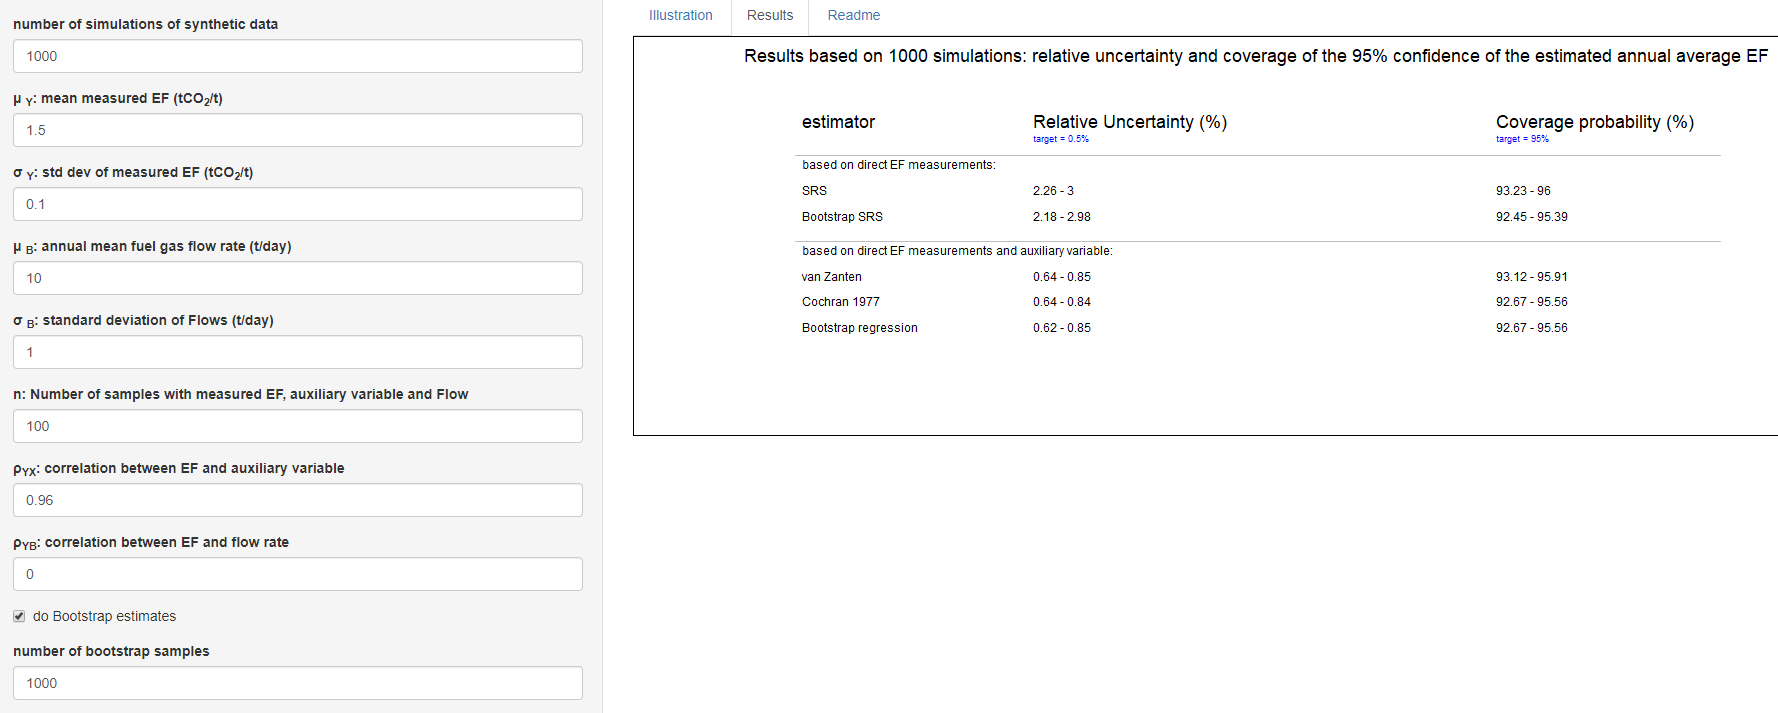
\includegraphics[width=\textwidth]{graphs/ResultsCapture.PNG}
	\caption{Screen shot of the web-App, with results. On the left are the inputs that define the scenario as well as the number of required simulations. On the right are the results in terms of the relative precisions and coverage probabilities. Note that these results took approximately 20 minutes to be generated. }
	\label{fig:AppResults}
\end{figure}


Another illustration of the results of the web-App, for a given scenario with $n=150$ and $\rho_{YX}=0.97$ is given in figure~\ref{fig:AppResults2}. For this particular scenario, the estimators with auxiliary variables (sections~\ref{AuxBoot},\ref{AuxCochran} and \ref{AuxVZ} all agree well in terms of both relative uncertainty and coverage, and yield uncertainty estimates in the range 0.46\% - 0.59\%; depending on chance the esitmate may come in just below or just above the target set by the NEA. 
\begin{figure}[h]
	\centering
	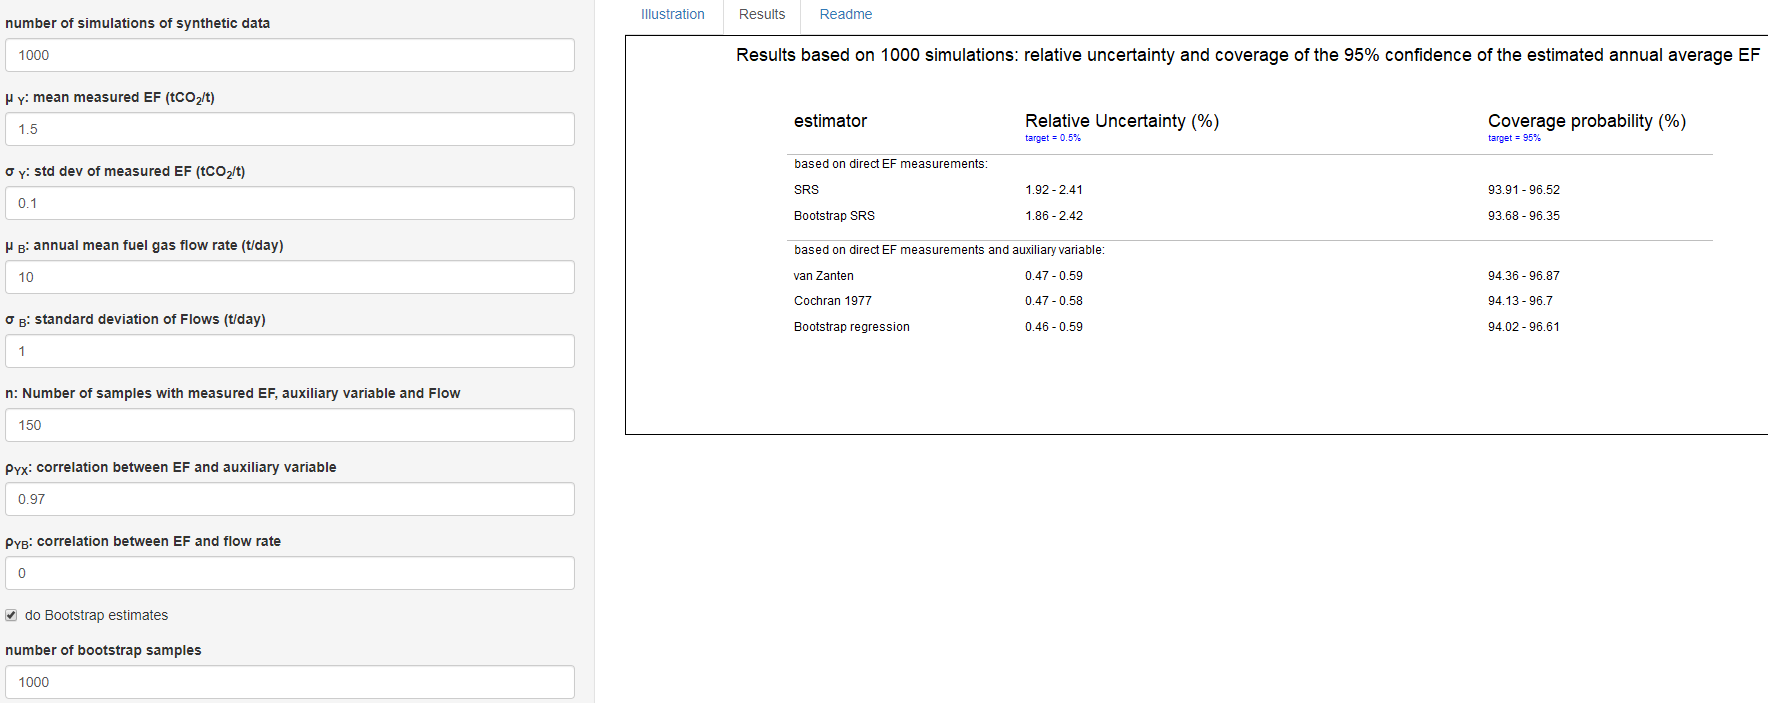
\includegraphics[width=\textwidth]{graphs/ResultsCapture2.PNG}
	\caption{Screen shot of the web-App, with results. On the left are the inputs that define the scenario as well as the number of required simulations. On the right are the results in terms of the relative precisions and coverage probabilities. Note that these results took approximately 20 minutes to be generated. }
	\label{fig:AppResults2}
\end{figure}

\clearpage
\section{Combining measurements from multiple fuel streams}\label{Combining}

If multiple fuel streams are sampled, then measurements may be combined to obtain an estimate of the average annual EF for all fuel streams combined. A lower relative uncertainty can be obtained if the measurements can be obtained. The statistical methodology, including the optimal allocation of sample sizes across fuel streams to minimize the relative uncertainty, is outlined in chapter 5.5 in \citet{Cochran77}.
%\clearpage
\section{Results of simulation study to assess the performance of estimators}\label{Results}

The performance of the estimators is assessed using simulation studies as described in chapter~\ref{Simulation}. A good estimator has high precision (small width of confidence interval) and good coverage probability.

A guide to the labels for estimators in graphs and tables:
\begin{itemize}
	\item SRS: Simple Random Sample estimator (section~\ref{SRS})
	\item Bootstrap SRS: simple Random Sample with Bootstrap (section~\ref{SRSBoot})
	\item Cochran 1977: Linear regression estimator (section~\ref{AuxCochran})
	\item van Zanten: van Zanten estimator (section~\ref{AuxVZ})
	\item Bootstrap regression: Linear regression estimator with Bootstrap (section~\ref{AuxBoot})
\end{itemize}

Estimators that do not rely on the bootstrap are computationally inexpensive, and can be applied quickly to a large number of synthetic data sets. This allows us to assess the coverage probability (a large number of trials is needed to get a reliable estimate) for a variety of scenarios. There are many scenarios that can be explored, and the web-App can be a suitable tool to do this. A number of scenarios are illustrated here. For each scenario, results are generated for a range of sample sizes and a range of correlations between auxiliary variable and EF. For all scenarios, the average EF and variability in EF are similar to that observed in the Pernis data ($\mu_y=1.5$ and $\sigma_y=0.1$; see chapter~\ref{Pernis}). For each scenario, the results are based on 2500 synthetic data sets: 
\begin{itemize}
	\item ``High variability in flow rates; no correlation between EF and flow rates'': figure~\ref{fig:Batch3}.
	\item ``Low variability in flow rates; no correlation between EF and flow rates'': figure~\ref{fig:Batch4}.
	\item ``High variability in flow rates; correlation between EF and flow rates'': figure~\ref{fig:Batch5}.
\end{itemize}

In all cases, the use of an auxiliary variable greatly improves the precision of the estimate of the annual average EF. The stronger the correlation between EF and auxiliary variable, the greater the increase in precision. As expected, precision increases as a function of sample size $n$. Increasing the variability in flow rate does not have a large impact on the precision of the estimate (compare figure~\ref{fig:Batch3} with figure~\ref{fig:Batch4}), but the coverage probability of the Cochran 1977 estimator is somewhat too low when the flow rates are highly variable. When the flow rate is correlated with the EF, the coverage probability of the Cochran 1977 estimator is somewhat too low, but the coverage probability of the van Zanten estimator is much too low (figure~\ref{fig:Batch5}). The standard of 0.5\% relative uncertainty can only be met with a combination of very strong correlation between auxiliary variable and large sample size. 

\begin{figure}[h]
	\centering
	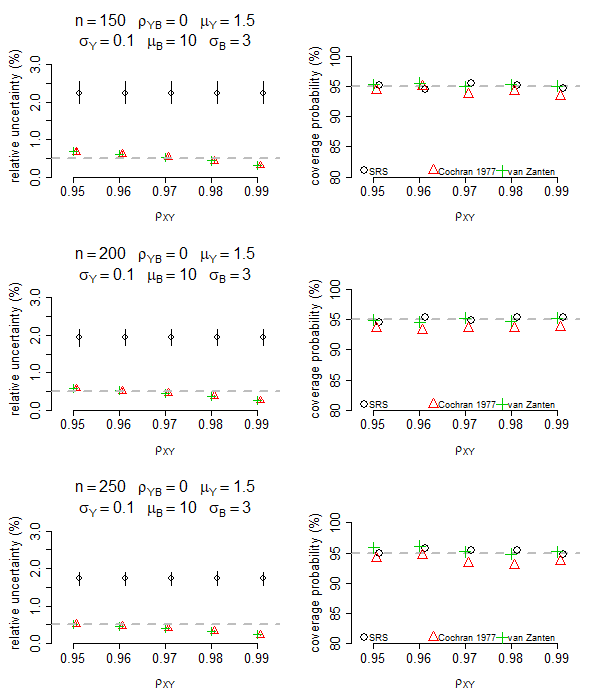
\includegraphics[width=\textwidth]{graphs/Results_Combined_withoutBoot_200.png}
	\caption{Relative uncertainty of the mean annual EF estimate, and coverage probability of the 95\% confidence interval, for the SRS, van Zanten and Cochran 1977 estimators. Scenario: no correlation between auxiliary variable and EF ($\rho_{YB}=0$), high variability in flow rates ($\mu_B=10$, $\sigma_B=3$). }
	\label{fig:Batch3}
\end{figure}

\begin{figure}[h]
	\centering
	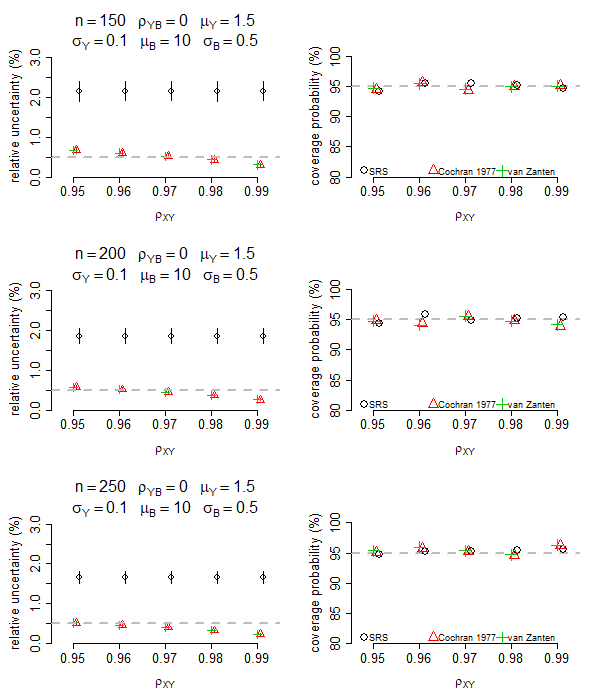
\includegraphics[width=\textwidth]{graphs/Results_Combined_withoutBoot_LowFlowRateVar250.png}
	\caption{Relative uncertainty of the mean annual EF estimate, and coverage probability of the 95\% confidence interval, for the SRS, van Zanten and Cochran 1977 estimators. Scenario: no correlation between auxiliary variable and EF ($\rho_{YB}=0$), low variability in flow rates ($\mu_B=10$, $\sigma_B=0.5$), no correlation between flow rate and EF ($\rho_{YB}$).}
	\label{fig:Batch4}
\end{figure}

\begin{figure}[h]
	\centering
	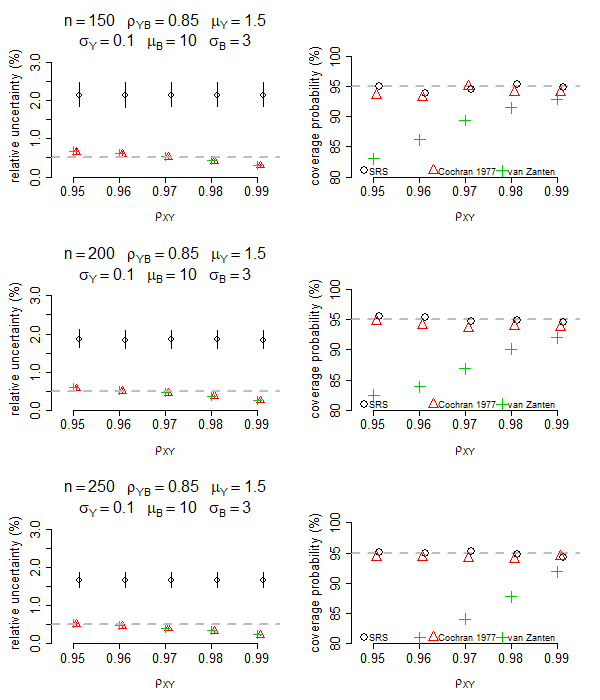
\includegraphics[width=\textwidth]{graphs/Results_Combined_withoutBoot_HighFlowRateVar_corB250.png}
	\caption{Relative uncertainty of the mean annual EF estimate, and coverage probability of the 95\% confidence interval, for the SRS, van Zanten and Cochran 1977 estimators. Scenario: strong correlation between auxiliary variable and EF ($\rho_{YB}=0.85$), high variability in flow rates ($\mu_B=10$, $\sigma_B=3$).}
	\label{fig:Batch5}
\end{figure}

The Bootstrap estimators are computationally intensive (see chapter~\ref{Estimators}), and a smaller number of  scenarios has been included for illustration here. For each scenario, the results are based on 2500 synthetic data sets: 
\begin{itemize}
	%\item Average and variability in EF similar to that observed in the Pernis fuel gas ($\mu_Y=1.5$, $\sigma_Y=0.1$), some variability in flow rates ($\mu_B=10$, $\sigma_B=1$), strong correlation between auxiliary variable and EF ($\rho_{YX}=0.96$) and no correlation between flow rate and EF ($\rho_{YB}=0$): table~\ref{tab:batch1}.
	\item Variability in EF similar to that observed in the Pernis fuel gas ($\mu_Y=1.5$, $\sigma_Y=0.1$), very high variability in flow rates ($\mu_B=10$, $\sigma_B=3$), strong correlation between auxiliary variable and EF ($\rho_{YX}=0.96$) and no correlation between flow rate and EF ($\rho_{YB}=0$): table~\ref{tab:batch2}.
	\item Variability in EF similar to that observed in the Pernis fuel gas ($\mu_Y=1.5$, $\sigma_Y=0.1$), very high variability in flow rates ($\mu_B=10$, $\sigma_B=3$), strong correlation between auxiliary variable and EF ($\rho_{YX}=0.96$) and strong correlation between flow rate and EF ($\rho_{YB}=0.85$): table~\ref{tab:batch3}.
	\item Variability in EF similar to that observed in the Pernis fuel gas ($\mu_Y=1.5$, $\sigma_Y=0.1$), low variability in flow rates ($\mu_B=10$, $\sigma_B=0.5$), very strong correlation between auxiliary variable and EF ($\rho_{YX}=0.99$) and no correlation between flow rate and EF ($\rho_{YB}=0.85$): table~\ref{tab:batch4}.
	\item Higher variability in EF similar compared to that observed in the Pernis fuel gas ($\mu_Y=1.5$, $\sigma_Y=0.15$), low variability in flow rates ($\mu_B=10$, $\sigma_B=0.5$), very strong correlation between auxiliary variable and EF ($\rho_{YX}=0.99$) and no correlation between flow rate and EF ($\rho_{YB}=0.85$): table~\ref{tab:batch5}.
\end{itemize}

The Bootstrap estimators yield very similar estimates of relative uncertainty compared to their analytical counterparts (compare SRS with Bootstrap SRS, and van Zanten or Cochran 1977 with Boostrap regression). When flow rate and EF are correlated, the van Zanten estimator has suboptimal coverage probability but the Bootstrap regression estimator performs well (table~\ref{tab:batch3} and ~\ref{tab:batch5}). The relative uncertainty is very low when the sample size is $n=200$ and when there is strong correlation between auxliary variable and EF ($\rho_{XY}=0.99$; table~\ref{tab:batch4}). the relative uncertainty increases substantially when the variability in EF increases (table~\ref{tab:batch5}).

%\begin{table}
%	\caption{Performance of estimators in a scenario with average and variability in EF similar to that observed in the Pernis fuel gas ($\mu_Y=1.5$, $\sigma_Y=0.1$),some variability in flow rates ($\mu_B=10$, $\sigma_B=1$), strong correlation between auxiliary variable and EF ($\rho_{YX}=0.96$) and no correlation between flow rate and EF ($\rho_{YB}=0$). }
%	\begin{tabular}{l l r@{.}l@{ - }r@{.}l r@{.}l@{ - }r@{.}l}
%		\hline
%		$n$ & Estimator & \multicolumn{4}{c}{Relative Uncertainty (\%)} & \multicolumn{4}{c}{Coverage probability (\%)} \\
%		\hline
%		100 & SRS 		 		& 2&30&3&01 & 93&01&95&83 \\
%		    & Bootstrap SRS 	& 2&23&2&99 & 92&87&95&65 \\
%		    & van Zanten   		& 0&64&0&85 & 94&25&96&78 \\
%		    & Cochran 1977 		& 0&64&0&84 & 93&97&96&52 \\
%		    & Boostrap regression & 0&62&0&85 & 93&79&96&44 \\
%		\cline{2-10}
%		200 & SRS 		 		& 1&64&2&05 & 93&23&96&00 \\
%		    & Bootstrap SRS 	& 1&65&2&06 & 93&01&95&83 \\
%		    & van Zanten   		& 0&47&0&58 & 94&70&97&12 \\
%		    & Cochran 1977 		& 0&47&0&57 & 94&59&97&04 \\
%		    & Boostrap regression & 0&46&0&58 & 94&59&97&04 \\
%		\hline
%	\end{tabular} \label{tab:batch1}
%\end{table}


\begin{table}
	\caption{Performance of estimators in a scenario with average and variability in EF similar to that observed in the Pernis fuel gas ($\mu_Y=1.5$, $\sigma_Y=0.1$), very high variability in flow rates ($\mu_B=10$, $\sigma_B=3$), strong correlation between auxiliary variable and EF ($\rho_{YX}=0.96$) and no correlation between flow rate and EF ($\rho_{YB}=0$).}
	\begin{tabular}{l l r@{.}l@{ - }r@{.}l r@{.}l@{ - }r@{.}l}
		\hline
		$n$ & Estimator & \multicolumn{4}{c}{Relative Uncertainty (\%)} & \multicolumn{4}{c}{Coverage probability (\%)} \\
		\hline
		100 & SRS 		 		& 2&33&3&26 & 94&02&96&61 \\
		    & Bootstrap SRS 	& 2&25&3&18 & 93&45&96&18 \\
		    & van Zanten   		& 0&64&0&85 & 93&45&96&18 \\
		    & Cochran 1977 		& 0&64&0&84 & 92&67&95&56 \\
		    & Boostrap regression & 0&62&0&85 & 92&45&95&39 \\
		\cline{2-10}
		200 & SRS 		 		& 1&73&2&05 & 93&79&96&44 \\
		    & Bootstrap SRS 	& 1&67&2&06 & 93&68&96&35 \\
		    & van Zanten   		& 0&47&0&58 & 95&05&97&38 \\
		    & Cochran 1977 		& 0&47&0&57 & 93&34&96&09 \\
		    & Boostrap regression & 0&46&0&58 & 94&25&96&78 \\
		\hline
	\end{tabular}\label{tab:batch2}
\end{table}

\begin{table}
	\caption{Performance of estimators in a scenario with average and variability in EF similar to that observed in the Pernis fuel gas ($\mu_Y=1.5$, $\sigma_Y=0.1$), very high variability in flow rates ($\mu_B=10$, $\sigma_B=3$), strong correlation between auxiliary variable and EF ($\rho_{YX}=0.96$) and strong correlation between flow rate and EF ($\rho_{YB}=0.85$).}
	\begin{tabular}{l l r@{.}l@{ - }r@{.}l r@{.}l@{ - }r@{.}l}
		\hline
		$n$ & Estimator & \multicolumn{4}{c}{Relative Uncertainty (\%)} & \multicolumn{4}{c}{Coverage probability (\%)} \\
		\hline 
		100 & SRS 		 		& 2&20&3&17 & 93&57&96&26 \\
		    & Bootstrap SRS 	& 2&13&3&15 & 93&12&95&91 \\
		    & van Zanten   		& 0&65&0&87 & 88&39&92&06 \\
		    & Cochran 1977 		& 0&63&0&83 & 92&34&95&30 \\
		    & Boostrap regression & 0&57&0&83 & 92&54&95&39 \\
		\cline{2-10}
		200 & SRS 		 		& 1&61&2&11 & 93&12&95&92 \\
		    & Bootstrap SRS 	& 1&56&2&10 & 92&23&95&21 \\
		    & van Zanten   		& 0&48&0&59 & 81&24&85&83 \\
		    & Cochran 1977 		& 0&46&0&56 & 92&89&95&74 \\
		    & Boostrap regression & 0&42&0&55 & 93&57&96&26 \\
		\hline
	\end{tabular}\label{tab:batch3}
\end{table}


\begin{table}
	\caption{Performance of estimators in a scenario with average and variability in EF similar to that observed in the Pernis fuel gas ($\mu_Y=1.5$, $\sigma_Y=0.1$), low variability in flow rates ($\mu_B=10$, $\sigma_B=0.5$), very strong correlation between auxiliary variable and EF ($\rho_{YX}=0.99$) and no correlation between flow rate and EF ($\rho_{YB}=0.85$).}
	\begin{tabular}{l l r@{.}l@{ - }r@{.}l r@{.}l@{ - }r@{.}l}
		\hline
		$n$ & Estimator & \multicolumn{4}{c}{Relative Uncertainty (\%)} & \multicolumn{4}{c}{Coverage probability (\%)} \\
		\hline
		100 & SRS 		 		& 2&28&3&01 & 93&01&95&83 \\
		    & Bootstrap SRS 	& 2&20&2&98 & 92&34&95&30 \\
		    & van Zanten   		& 0&32&0&43 & 94&25&96&78 \\
		    & Cochran 1977 		& 0&32&0&43 & 94&47&96&95 \\
		    & Boostrap regression & 0&31&0&43 & 94&25&96&30 \\
		\cline{2-10}
		200 & SRS 		 		& 1&68&2&05 & 93&91&96&52 \\
		    & Bootstrap SRS 	& 1&63&2&05 & 92&12&95&91 \\
		    & van Zanten   		& 0&24&0&29 & 93&79&96&44 \\
		    & Cochran 1977 		& 0&24&0&29 & 93&68&96&35 \\
		    & Boostrap regression & 0&23&0&29 & 93&57&96&26 \\
		\hline
	\end{tabular}\label{tab:batch4}
\end{table}


\begin{table}
	\caption{Performance of estimators in a scenario with higher variability in EF similar compared to that observed in the Pernis fuel gas ($\mu_Y=1.5$, $\sigma_Y=0.15$), low variability in flow rates ($\mu_B=10$, $\sigma_B=0.5$), very strong correlation between auxiliary variable and EF ($\rho_{YX}=0.99$) and no correlation between flow rate and EF ($\rho_{YB}=0.85$).}
	\begin{tabular}{l l r@{.}l@{ - }r@{.}l r@{.}l@{ - }r@{.}l}
		\hline
		$n$ & Estimator & \multicolumn{4}{c}{Relative Uncertainty (\%)} & \multicolumn{4}{c}{Coverage probability (\%)} \\
		\hline
		100 & SRS 		 		& 3&38&4&52 & 92&67&95&56 \\
		    & Bootstrap SRS 	& 3&72&4&46 & 91&67&94&76 \\
		    & van Zanten   		& 0&49&0&65 & 92&00&95&03 \\
		    & Cochran 1977 		& 0&49&0&65 & 91&34&94&50 \\
	        & Boostrap regression & 0&47&0&65 & 92&00&95&03 \\
		\cline{2-10}
		200 & SRS 		 		& 2&52&3&07 & 94&13&96&70 \\
		    & Bootstrap SRS 	& 2&45&3&06 & 93&97&96&52 \\
		    & van Zanten   		& 0&36&0&44 & 93&45&96&18 \\
		    & Cochran 1977 		& 0&35&0&43 & 93&01&95&83 \\
		    & Boostrap regression & 0&35&0&44 & 92&78&95&65 \\
		\hline
	\end{tabular}\label{tab:batch5}
\end{table}




%\begin{table}
%	\caption{Scenario 1: $\mu_Y=1.5$, $\sigma_Y=0.1$, $\mu_B=10$, $\sigma_B=1$, $\rho_{YX}=0.96$, $\rho_{YB}=0$. Scenario 2: $\mu_Y=1.5$, $\sigma_Y=0.1$, $\mu_B=10$, $\sigma_B=3$, $\rho_{YX}=0.96$, $\rho_{YB}=0$. Scenario 3: $\mu_Y=1.5$, $\sigma_Y=0.1$, $\mu_B=10$, $\sigma_B=3$, $\rho_{YX}=0.96$, $\rho_{YB}=0.85$. Scenario 4: $\mu_Y=1.5$, $\sigma_Y=0.1$, $\mu_B=10$, $\sigma_B=0.5$, $\rho_{YX}=0.99$, $\rho_{YB}=0$. Scenario 5: $\mu_Y=1.5$, $\sigma_Y=0.15$, $\mu_B=10$, $\sigma_B=0.5$, $\rho_{YX}=0.99$, $\rho_{YB}=0$.}
%	\begin{tabular}{l l l r@{.}l@{ - }r@{.}l r@{.}l@{ - }r@{.}l}
%		\hline \hline
%		Scenario & $n$ & Estimator & \multicolumn{4}{c}{Relative Uncertainty (\%)} & \multicolumn{4}{c}{Coverage probability (\%)} \\
%		\hline
%		1   & 100 & SRS 		 		& 2&30&3&01 & 93&01&95&83 \\
%		& 	  & Bootstrap SRS 		& 2&23&2&99 & 92&87&95&65 \\
%		& 	  & van Zanten   		& 0&64&0&85 & 94&25&96&78 \\
%		&     & Cochran 1977 		& 0&64&0&84 & 93&97&96&52 \\
%		&	  & Boostrap regression & 0&62&0&85 & 93&79&96&44 \\
%		\cline{2-11}
%		& 200 & SRS 		 		& 1&64&2&05 & 93&23&96&00 \\
%		& 	  & Bootstrap SRS 		& 1&65&2&06 & 93&01&95&83 \\
%		& 	  & van Zanten   		& 0&47&0&58 & 94&70&97&12 \\
%		&     & Cochran 1977 		& 0&47&0&57 & 94&59&97&04 \\
%		&	  & Boostrap regression & 0&46&0&58 & 94&59&97&04 \\
%		\hline 
%		2   & 100 & SRS 		 		& 2&33&3&26 & 94&02&96&61 \\
%		& 	  & Bootstrap SRS 		& 2&25&3&18 & 93&45&96&18 \\
%		& 	  & van Zanten   		& 0&64&0&85 & 93&45&96&18 \\
%		&     & Cochran 1977 		& 0&64&0&84 & 92&67&95&56 \\
%		&	  & Boostrap regression & 0&62&0&85 & 92&45&95&39 \\
%		\cline{2-11}
%		& 200 & SRS 		 		& 1&73&2&05 & 93&79&96&44 \\
%		& 	  & Bootstrap SRS 		& 1&67&2&06 & 93&68&96&35 \\
%		& 	  & van Zanten   		& 0&47&0&58 & 95&05&97&38 \\
%		&     & Cochran 1977 		& 0&47&0&57 & 93&34&96&09 \\
%		&	  & Boostrap regression & 0&46&0&58 & 94&25&96&78 \\
%		\hline 
%		3   & 100 & SRS 		 		& 2&20&3&17 & 93&57&96&26 \\
%		& 	  & Bootstrap SRS 		& 2&13&3&15 & 93&12&95&91 \\
%		& 	  & van Zanten   		& 0&65&0&87 & 88&39&92&06 \\
%		&     & Cochran 1977 		& 0&63&0&83 & 92&34&95&30 \\
%		&	  & Boostrap regression & 0&57&0&83 & 92&54&95&39 \\
%		\cline{2-11}
%		& 200 & SRS 		 		& 1&61&2&11 & 93&12&95&92 \\
%		& 	  & Bootstrap SRS 		& 1&56&2&10 & 92&23&95&21 \\
%		& 	  & van Zanten   		& 0&48&0&59 & 81&24&85&83 \\
%		&     & Cochran 1977 		& 0&46&0&56 & 92&89&95&74 \\
%		&	  & Boostrap regression & 0&42&0&55 & 93&57&96&26 \\
%		\hline 
%		4   & 100 & SRS 		 		& 2&28&3&01 & 93&01&95&83 \\
%		& 	  & Bootstrap SRS 		& 2&20&2&98 & 92&34&95&30 \\
%		& 	  & van Zanten   		& 0&32&0&43 & 94&25&96&78 \\
%		&     & Cochran 1977 		& 0&32&0&43 & 94&47&96&95 \\
%		&	  & Boostrap regression & 0&31&0&43 & 94&25&96&30 \\
%		\cline{2-11}
%		& 200 & SRS 		 		& 1&68&2&05 & 93&91&96&52 \\
%		& 	  & Bootstrap SRS 		& 1&63&2&05 & 92&12&95&91 \\
%		& 	  & van Zanten   		& 0&24&0&29 & 93&79&96&44 \\
%		&     & Cochran 1977 		& 0&24&0&29 & 93&68&96&35 \\
%		&	  & Boostrap regression & 0&23&0&29 & 93&57&96&26 \\
%		\hline 
%		5   & 100 & SRS 		 		& 3&38&4&52 & 92&67&95&56 \\
%		& 	  & Bootstrap SRS 		& 3&72&4&46 & 91&67&94&76 \\
%		& 	  & van Zanten   		& 0&49&0&65 & 92&00&95&03 \\
%		&     & Cochran 1977 		& 0&49&0&65 & 91&34&94&50 \\
%		&	  & Boostrap regression & 0&47&0&65 & 92&00&95&03 \\
%		\cline{2-11}
%		& 200 & SRS 		 		& 2&52&3&07 & 94&13&96&70 \\
%		& 	  & Bootstrap SRS 		& 2&45&3&06 & 93&97&96&52 \\
%		& 	  & van Zanten   		& 0&36&0&44 & 93&45&96&18 \\
%		&     & Cochran 1977 		& 0&35&0&43 & 93&01&95&83 \\
%		&	  & Boostrap regression & 0&35&0&44 & 92&78&95&65 \\
%		\hline 	\hline
%	\end{tabular}
%\end{table}
\clearpage
\section{Data analysis Pernis Refinery}\label{Pernis}
In this section, a descriptive analysis of EF measurements from a fuel gas in the Pernis refinery is presented. 
From 2014 to 2020, the fuel gas stream has been sampled at more or less regular intervals albeit with certain longer periods without any measurements. For each sample, the EF is measured based on a full analysis of the composition of the fuel gas in the laboratory. There is considerable variability in the EF over time (figure~\ref{fig:timeseries}), which is believed to be a reflection of the variability in process conditions, as the measurement uncertainty is small. The annual variability in EF, due to temporal variability in the composition of the fuel gas, is given in figure~\ref{fig:Pernis_hist}.

\begin{figure}[h]
	\centering
	\includegraphics[width=0.65\textwidth]{graphs/timeseries.pdf}
	\caption{Time series plot of EF, measured on samples taken from the flow of a fuel gas at the Pernis refinery.}
	\label{fig:timeseries}
\end{figure}

\begin{figure}[h]
	\centering
	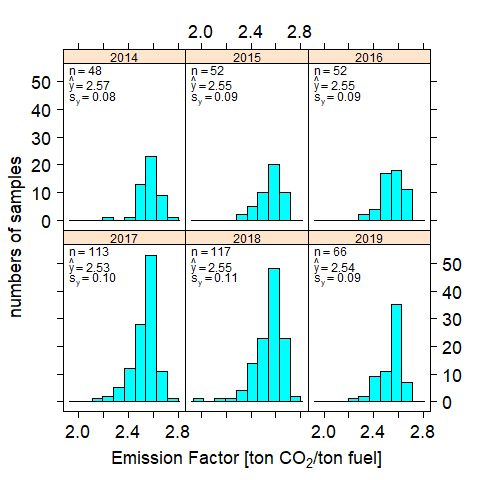
\includegraphics[width=0.65\textwidth]{graphs/Pernis_hist.pdf}
	\caption{Frequency histograms of EF, measured on samples taken from the flow of a fuel gas at the Pernis refinery. Indicated are the annual number of samples $n$, the annual standard deviation in measured EF ($\sigma_y$) and the annual average EF ($\hat{y}$).}
	\label{fig:Pernis_hist}
\end{figure}

The EF correlates very strongly with the Stoichiometric Air Requirement (SAR; figure~\ref{fig:SAR_y_peryear}) and less strongly with Lower Heating Value (LHV; figure~\ref{fig:LHV_y_peryear}). Estimates of SAR and LHV are based on the composition of the sample of fuel gas as determined in the laboratory. As such, these variables are therefore not directly useful as auxiliary variables. However, these relationships may provide clues to potential candidates for high-frequency online measurements that may correlate well with EF. SAR may be directly estimated based on a mass spectrometry device (see e.g. \cite{Merriman}), and it is worth investigating if oxygen analyzers or calorimeters correlate well with either SAR or LHV.

\begin{figure}[h]
	\centering
	\includegraphics[width=0.65\textwidth]{graphs/SAR_y_peryear.pdf}
	\caption{Scatterplot of EF against Stoichiometric Air Requirement (SAR), with Pearson correlation coefficients ($\rho$). }
	\label{fig:SAR_y_peryear}
\end{figure}


\begin{figure}[h]
	\centering
	\includegraphics[width=0.65\textwidth]{graphs/LHV_y_peryear.pdf}
	\caption{Scatterplot of EF against Lower Heating Value (LHV), with Pearson correlation coefficients ($\rho$). }
	\label{fig:LHV_y_peryear}
\end{figure}

%\begin{figure}[h]
%	\centering
%	\includegraphics[width=0.7\textwidth]{graphs/SAR_y_residuals.pdf}
%	\caption{ }
%	\label{fig:SAR_y_residuals}
%\end{figure}
The residuals of a linear model of EF on SAR correlate strongly with molar weight as measured by an analyser which is already online in the fuel gas stream at the Pernis refinery (figure~\ref{fig:SAR_y_residuals_molweight_peryear}). A multiple linear regression model of EF on SAR and molar weight yields predictions that correlate very strongly with measured EF (figure~\ref{fig:SAR_y_predicted_SAR_molweight_peryear}). This is encouraging because, if a device can be found which can measure online a variable which correlates with SAR or LHV, then this may result in a model with good predictive performance in combination with online molar weight measurements.

\begin{figure}[h]
	\centering
	\includegraphics[width=0.65\textwidth]{graphs/SAR_y_residuals_molweight_peryear.pdf}
	\caption{ Scatterplot of the residuals of a linear regression model of EF on SAR, versus molar weight. }
	\label{fig:SAR_y_residuals_molweight_peryear}
\end{figure}

\begin{figure}[h]
	\centering
	\includegraphics[width=0.65\textwidth]{graphs/SAR_y_predicted_SAR_molweight_peryear.pdf}
	\caption{Scatterplot of measured versus predicted EF. The EF was predicted using a linear regression model with SAR and molar weight as covariates. Indicated on the graphs are Pearson correlation coefficients ($\rho$). }
	\label{fig:SAR_y_predicted_SAR_molweight_peryear}
\end{figure}

A time series plot of the residuals of the multiple linear regression model of EF on SAR and molar weight indicates that there are still some unexplained trends in the EF measurements (figure~\ref{fig:SAR_residuals_SAR_molweight_timeseries}). For example, there is a consistent deviation between predicted and measured EF in 2019. This, however, does not have to lead to a deterioration of the uncertainty of the estimate of the annual average, as long as the annual average EF is based on a combination of direct EF measurements in the laboratory and the auxiliary variable(s).

\begin{figure}[h]
	\centering
	\includegraphics[width=0.65\textwidth]{graphs/SAR_residuals_SAR_molweight_timeseries.pdf}
	\caption{Time series plot of the residuals of a multiple linear regression model of EF on SAR and molar weight. }
	\label{fig:SAR_residuals_SAR_molweight_timeseries}
\end{figure}

An exploratory data analysis (not shown in this report) indicated that the residuals of the multiple linear regression model of EF on SAR and molar weight correlate with ethylene and propylene concentrations in the fuel gas. Based on these two additional variables, the predictive model for EF could be further improved. However, this is not further discussed or illustrated here.
%
%\begin{figure}[h]
%	\centering
%	\includegraphics[width=0.65\textwidth]{graphs/SAR_y_predicted_SAR_molweight_Pr_Eth_peryear.pdf}
%	\caption{ }
%	\label{fig:SAR_y_predicted_SAR_molweight_Pr_Eth_peryear}
%\end{figure}
%
%\begin{figure}[h]
%	\centering
%	\includegraphics[width=0.65\textwidth]{graphs/Residuals_SAR_molweight_Pr_Eth_timeseries.pdf}
%	\caption{ }
%	\label{fig:Residuals_SAR_molweight_Pr_Eth_timeseries}
%\end{figure}

%\clearpage
\section{Summary of main Results}\label{Discussion}
A number of statistical procedures (estimators) for estimating the mean annual EF as well as the relative uncertainty of the estimate of the mean, have been described and assessed using a simulation study. The aim was to better understand the performance of these estimators, in terms of their relative uncertainties and coverage probabilities, under different scenarios for variability in EF measurements, flow rates, sample sizes and correlations between the key variables.

The main learnings are:
\begin{itemize}
	\item The use of an auxiliary variable has the potential to greatly increase the precision of the estimate of the annual average EF. In order to obtain very high precision of estimates, for example less than 0.5\% relative uncertainty, it is necessary to have an auxiliary variable which correlates strongly with EF measurements.
	\item Without an auxiliary variable, a large number of samples is required to get high precision.
	\item A simulation tool has been developed in an App that can be used to find the required sample size to obtain a specified precision, as a function of the main variables of interest: process variability in EF, variability in flow rates and correlations between the variables of interest. The parameters can be estimated from actual process data. An example from a fuel gas in the Pernis refinery is included,
	\item Estimators based on auxiliary variables are model based, so model checking is required as outlined in \citet{vanZanten} and in chapter~\ref{Validation}.
	\item The van Zanten estimator has good performance and good coverage probability, except when the variability in flow rate is high and the flow rate is correlated with EF.
	\item The coverage of the linear regression estimator is slightly too low if the variability in flow rates is high. The performance of the linear regression estimator does not deteriorate when there is a correlation between flow rate and EF.
	\item The Bootstrap estimators have good performance, and can readily be extended to multiple regression, or other types of relationships of needed.
	\item The following factors have a particularly large influence on the relative uncertainty:
	\begin{itemize}
		\item The sample size $n$ (number of laboratory measurements on samples taken from the flow of the fuel gas): the larger the sample size, the smaller the relative uncertainty.
		\item The process variability in EF $\sigma_Y$: the larger the process variability in EF the larger the relative uncertainty.
		\item The correlation between the auxiliary variable and EF $\rho_{XY}$: the stronger the correlation (the closer it is to 1) the lower the relative uncertainty.
	\end{itemize}
\end{itemize}

If there is a single auxiliary variable and there is no correlation between flow rate and EF, then the van Zanten estimator is appropriate if the other assumptions that apply to this method are reasonable (see \citet{vanZanten} and chapter~\ref{Validation}).
If, in addition to the above, the variability in flow rates is low, then the regression estimator from \citet{Cochran77} is also acceptable. This estimator has the advantage that it is described in textbooks and is easy to understand.

The Bootstrap methods also perform well, and have the advantage that they can be readily extended to other situation, in particular for multiple regression when multiple auxiliary variables are available. A disadvantage of the Bootstrap is that it can only be implemented using specialist statistical software.

An analysis of data from a fuel gas in the Pernis refinery indicates a number of potential candidates for auxiliary variables. A multiple linear regression model of EF on Stoichiometric Air Requirement (SAR) or Lower Heating Value (LHV) and molar weight yields predictions that correlate very strongly with measured EF (figure~\ref{fig:SAR_y_predicted_SAR_molweight_peryear}). This is encouraging because, if a device can be found which can measure online a variable which correlates with SAR or LHV, then this may result in a model with good predictive performance in combination with online molar weight measurements.


\clearpage
\bibliography{ref}
\clearpage


\end{document}